\chapter{Implications for model evaluation}\label{sec:cmip5}

With the uncertainty analysis in Section~\ref{sec:misr} and the
identification in Section~\ref{sec:subgrid1} and
Section~\ref{sec:subgrid2} of potential ambiguities in results due to
treatments of unresolved clouds and precipitation in simulating
satellite diagnostics from COSP, the question remains: what conclusions
can be robustly determined by comparing clouds retrieved from space with
simulated views of clouds from space? In other words, which differences
identified between modeled and observed cloud statistics can be
attributed to model biases, as opposed to limitations or errors in the
current framework? This question is addressed in this chapter in the
context of an inter-comparison of cloud and radiative flux statistics in
a selection of five different global climate models, which all
participated in CMIP5/CFMIP2.

\section{Models and observations}\label{models-and-observations}

Five models are compared in this study using COSP output generated from
the inline implementation of COSP within each model: the Geophysics
Fluid Dynamics Laboratory (GFDL) AM3 \citep{donner_et_al_2011}, the
National Center for Atmospheric Research (NCAR) CAM4
\citep{neale_et_al_2010a} and CAM5 \citep{neale_et_al_2010b}, the
Canadian Centre for Climate Modeling and Analysis (CCCma) CanAM4
\citep{von_salzen_et_al_2012}, and the UK Met Office Hadley Center
(MOHC) HadGEM2 \citep{martin_et_al_2011}. These models are the
atmosphere-only components of the fully-coupled earth system models
produced by each respective institution. The simulations presented here
were run in ``AMIP'' configuration {[}citations{]}, in which the model
is forced by observed sea-surface-temperatures and run without an
interactive ocean component.

The analysis presented here compares simulated views of clouds from COSP
between models and against satellite retrievals, and connects identified
biases in cloud statistics with biases in cloud radiative effects. Each
of the models evaluated here have included COSP into their source code,
and COSP outputs were generated by running COSP inline with the model
for the length of the simulation time.

Each of the participating modeling centers have provided both the MISR
and ISCCP-simulated cloud top height (or pressure) and optical depth
(CTH-OD or CTP-OD) joint histogram outputs from COSP. These outputs are
evaluated against the corresponding CTH-OD and CTP-OD datasets produced
by the MISR and ISCCP science teams, available as monthly-mean gridded
products from the CFMIP archive\footnote{http://climserv.ipsl.polytechnique.fr/cfmip-obs/}.
These datasets are briefly summarized here, and a more comprehensive
description can be found in \citet{marchand_et_al_2010}.

As discussed in Section~\ref{sec:misr}, the MISR instrument has a unique
arrangement of nine different cameras, each pointed at a different
viewing angle along the satellite track. The successive imaging of cloud
scenes from different angles allows MISR to use a stereo imaging
technique to retrieve cloud top heights (\(z_c\)) as opposed to the
cloud brightness temperature technique used by ISCCP and other
single-camera radiometer-based retrievals
\citep{moroney_et_al_2002, muller_et_al_2002}. One of the consequences
of this is that MISR sees through optically thin, high-level clouds and
retrieves the cloud otp height of the underlying cloud layer in cases of
multi-layered cloud scenes involving optically thin high-level cloud
over an optically thicker cloud layer \citep{marchand_et_al_2010}. Thus,
low-topped cloud amounts from MISR tend to be larger than those from
ISCCP, while mid and high-topped cloud amounts tend to be smaller. For
MISR, low-topped clouds are defined as those with \(z_c < 3\) km,
mid-topped clouds are defined as those with \(3 < z_c < 7\) km, and
high-topped clouds are defined as those with \(z_c > 7\) km.

Radiative fluxes are evaluated against the Clouds and the Earths Radiant
Energy Balanced and Filled dataset \citep[CERES-EBAF Version
2.6;][]{loeb_et_al_2009}. This dataset was developed specifically for
climate model evaluation. The shortwave and longwave fluxes in this
dataset have been adjusted within the observational uncertainty to
obtain a net top of atmosphere (TOA) energy balance that ismore
consistent with estimates of global heat storage. The CERES-EBAF dataset
covers the time period from the year 2000 to present, and is available
directly from the CERES team\footnote{https://ceres-tool.larc.nasa.gov/ord-tool/srbavg},
or from CFMIP in gridded, monthly averaged form\footnote{http://climserv.ipsl.polytechnique.fr/cfmip-obs/}.

The instantaneous effect of clouds on the TOA radiation budget can be
quantified by calculating the difference between the all-sky and
clear-sky fluxes
\citep[e.g.,][]{ellis_and_vonderhaar_1976, ramanathan_1987, ramanathan_et_al_1989}.
In this context, clear-sky means non-cloudy, so aerosol effects are
implicitely contained in the clear-sky fluxes. The resulting quantity is
commonly referred to as the cloud radiative forcing or CRF. This
language is somewhat misleading, however, as this quantity is not
strictly a forcing, but rather a measure of the effect of clouds on the
instantaneous TOA fluxes \citep{stephens_2005}. A more appropriate term
for this quantity is the cloud radiative effect, or simply the CRE, and
it will be referred as such here. The CRE can be calculated separately
for the shortwave and longwave fluxes, and model biases will be
evaluated separately in each of these broad spectral bands here.

Because MISR cloud optical depths are not computed over land or ice,
MISR comparisons can only be made over ice-free oceans. Thus, all model
output is masked consistent with MISR before making comparisons with
MISR cloud area. Both observations and models are averaged over the
period from 2001 to 2008, which is the largest period for which
observations and model output are available from each dataset and model.
All observations and data are regridded (using bi-linear interpolation)
to a common 2.5 degree by 2.5 degree regular latitude-longitude grid.

\section{Biases in CMIP5 models relative to satellite
retrievals}\label{biases-in-cmip5-models-relative-to-satellite-retrievals}

Figure~\ref{fig:cmip5_cldmisr_maps} shows climatological-mean
MISR-retrieved cloud area by cloud type and MISR-simulated cloud area by
cloud top height from each of the five models. The global
(area-weighted) means are summarized in Table~\ref{tbl:cmip5_cldmisr},
and differences between each of the models and the MISR retrievals
(calculated as model minus MISR) are shown in
Figure~\ref{fig:cmip5_cldmisr_maps_diff}.
Figure~\ref{fig:cmip5_cldmisr_maps} shows that each model is able to
capture the broad spatial patterns of cloudiness retrieved by MISR,
including the large amounts of high-topped cloud in the tropical
pacific, the subtropical coastal marine stratocumulus, the relatively
small cloud total cloud amounts inthe subtropical dry zones, and the
generally large total cloud amounts in the southern ocean.
Table~\ref{tbl:cmip5_cldmisr} suggests that total cloud cover is
universally underestimated in the models relative to the MISR
retrievals, however, with globally averaged differences between 6\% (for
AM3) and 25\% (for CAM4) cloud area (or 8\% to 35\% relative error).
Much of this apparent error is due to differences in low-topped cloud
area, and Figure~\ref{fig:cmip5_cldmisr_maps_diff} shows that low-topped
cloud differences (and indeed much of the total cloud differences) are
largest throughout the subtropics, where subtropical stratocumulus and
trade cumulus are dominant cloud types. As discussed in Chapter 2, the
broken nature of these cloud types makes determination of cloud area as
retrieved by an imager like MISR with a large field of view in relation
to the size of cloud elements problematic and somewhat ambiguous, as
cloud area is inherently tied to imager resolution for broken cloud
scenes. Thus, much of these differences in total cloud area are likely
due to systematic biases in MISR cloud detection and ``pixel-filling''
in cases of many small, broken clouds. It was estimated in Chapter 2
that this effect likely accounts for about 10\% of these differences
(see, e.g., Figure~\ref{fig:misr_rlmask_test}). While this effect can
explain much of these differences, errors in CAM4, CAM5, and HadGEM2
total cloud area are in excess of 10\%, and low-topped errors in CAM4
and HadGEM2 in particular are likewise in excess of 10\%. These errors
are larger than expected due to errors in the MISR cloud detection alone
and likely represent actual model biases, while the total cloud
differences in the remaining models cannot be ruled out as resulting
from errors in the MISR cloud detection.

\begin{figure}[htbp]
\centering
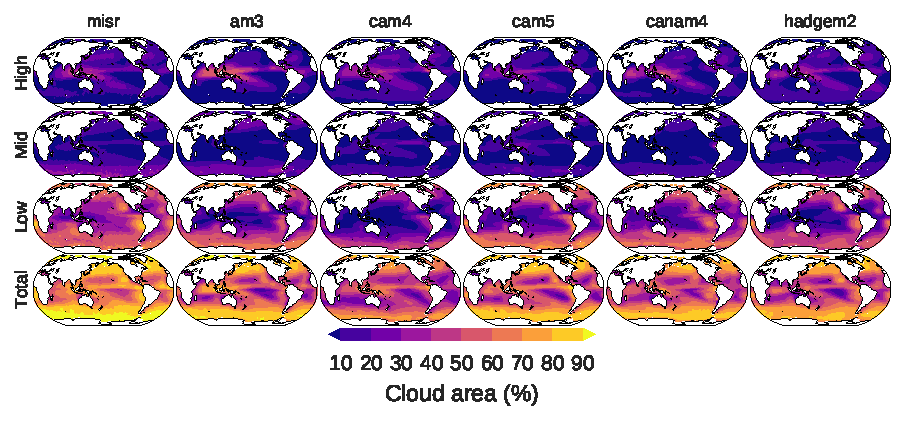
\includegraphics{graphics/cmip5_cldmisr.pdf}
\caption{\label{fig:cmip5_cldmisr_maps}MISR and MISR-simulated total,
high-topped, mid-topped, and low-topped cloud area in each of the five
models and from MISR retrievals. Global means are shown in
Table~\ref{tbl:cmip5_cldmisr}}\label{fig:cmip5ux5fcldmisrux5fmaps}
\end{figure}

\begin{figure}[htbp]
\centering
\includegraphics{graphics/cmip5_cldmisr_diff.pdf}
\caption{\label{fig:cmip5_cldmisr_maps_diff}Difference in MISR-simulated
total, high-topped, mid-topped, and low-topped cloud area in each of the
five models relative to MISR
retrievals.}\label{fig:cmip5ux5fcldmisrux5fmapsux5fdiff}
\end{figure}

Globally averaged differences for high and mid-topped cloud area are as
large as -5\% (CanAM4) cloud area (-42\% relative error), but these
errors are all within the uncertainties in MISR comparisons using the
simulator framework identified in Chapter 2, and thus should not be
interpreted alone as model biases. However,
Figure~\ref{fig:cmip5_cldmisr_maps_diff} shows that regional errors in
mid and high-topped cloud can exceed these ranges by a sizeable margin,
with high-topped cloud area differences relative to MISR exceeding 20\%
cloud area throughout the tropical western pacific in AM3 and CanAM4.
While these differences are much larger than can be explained by
inherent biases in the MISR retrieval, they are of the same sign and of
comparable magnitude to the errors identified in Chapter 3 that result
from assuming homogeneous cloud condensate amounts in generating
stochastic subcolumns for use with the simulators. Those errors inherent
in the subcolumn generator were estimated to result in errors in excess
of 10\% cloud area throughout the same tropical deep convective regions
identified as having large errors in high-topped cloud in the AM3 and
CanAM4 models. This suggests that much of the error in AM3 and CanAM4
high-topped cloud in the tropical western pacific may be at least
partially a result of assuming homogeneous cloud condensate in the
diagnostic code, rather than due to inherent model biases alone.

\begin{longtable}[]{@{}lcccccc@{}}
\caption{\label{tbl:cmip5_cldmisr}Globally-averaged cloud area by cloud
type from MISR observations and from the MISR simulator output from AM3,
CAM4, CAM5, CanAM4, and HadGEM2. }\tabularnewline
\toprule
Cloud type & MISR & AM3 & CAM4 & CAM5 & CanAM4 & HadGEM2\tabularnewline
\midrule
\endfirsthead
\toprule
Cloud type & MISR & AM3 & CAM4 & CAM5 & CanAM4 & HadGEM2\tabularnewline
\midrule
\endhead
High & 13 & 14 & 15 & 10 & 13 & 14\tabularnewline
Mid & 12 & 9 & 9 & 9 & 7 & 9\tabularnewline
Low & 43 & 32 & 20 & 35 & 35 & 30\tabularnewline
Total & 71 & 58 & 46 & 57 & 55 & 54\tabularnewline
\bottomrule
\end{longtable}

The more egregious of the model errors in cloud area manifest as errors
in cloud radiative effects as well. Figure~\ref{fig:cmip5_cre_maps}
shows cloud radiative effects from CERES-EBAF and from each of the
models, and Figure~\ref{fig:cmip5_cre_maps_diff} shows differences
between each model and CERES-EBAF (calculated as model minus
CERES-EBAF). Figure~\ref{fig:cmip5_cre_maps} shows that models tend to
capture the broad spatial patterns in shortwave, longwave, and net cloud
radiative effect, but Figure~\ref{fig:cmip5_cre_maps_diff} shows large
errors that have similarities to the errors in MISR-simulated cloud
area. In particular, AM3, CAM4, and CanAM4 have large errors in longwave
cloud radiative effect throughout the tropical western pacific (on the
order of 20 \(\textrm{W}/\textrm{m}^2\)). These errors are consistent
with the overestimate from these models in high-topped (and mid-topped)
cloud area relative to MISR identified in
Figure~\ref{fig:cmip5_cldmisr_maps_diff}, since high-topped cloud is
most relevant to the longwave (cooling) cloud radiative effect. That
these errors exist in both cloud radiative effect and in cloud area
gives further confidence to the results obtained in
Figure~\ref{fig:cmip5_cldmisr_maps_diff}, but this also raises further
concern about the treatment of cloud properties in models. The
similarities between longwave cloud radiative effect errors,
MISR-simulated high-topped cloud area errors, and the errors that
resulted from homogenizing cloud condensate in Chapter 3 suggest again
that these errors are likely due at least in part to the assumption of
homogeneous cloud condensate in the radiative transfer code in these
models.

\begin{figure}[htbp]
\centering
\includegraphics{graphics/cmip5_cre_maps.pdf}
\caption{\label{fig:cmip5_cre_maps}Shortwave (top), longwave (middle)
and net (bottom) cloud radiative effects from CERES-EBAF (left) and from
each of the five models evaluated in this study (from left to right,
AM3, CAM4, CAM5, CanAM4, HadGEM2). Numbers in the lower right corner of
each map indicate the area-weighted global
mean.}\label{fig:cmip5ux5fcreux5fmaps}
\end{figure}

\begin{figure}[htbp]
\centering
\includegraphics{graphics/cmip5_cre_maps_diff.pdf}
\caption{\label{fig:cmip5_cre_maps_diff}Differences in shortwave (top),
longwave (middle) and net (bottom) cloud radiative effects in each of
the five models relative to CERES-EBAF, calculated as model minus
observations. Numbers in the lower right corner of each map indicate the
area-weighted global mean of the
difference.}\label{fig:cmip5ux5fcreux5fmapsux5fdiff}
\end{figure}

\section{Summary, discussion, and future
directions}\label{summary-discussion-and-future-directions}

In this chapter, differences between a selection of GCM-simulated cloud
properties and satellite-retrieved cloud properties from MISR and
CloudSat have been quantified. Differences between models and
observations are often taken at face value to represent model biases,
but the results from Chapters 2, 3, and 4 suggest that more care must be
taken to properly interpret these differences. The purpose of this
chapter is to illustrate the pitfalls in interpreting these differences,
with the additional benefit of identifying model biases that cannot be
entirely explained by limitations in the comparison framework and thus
likely represent model parameterization errors.

Low-topped and total cloud area is universally underestimated in the
models considered here relative to MISR retrievals, but most of these
differences are consistent with expectations for MISR to overestimate
the true cloud area due to resolution effects. In particular, model
underestimates of low-topped cloud throughout the subtropics likely
represent primarily this feature of available imager retrievals of cloud
area, rather than inherent model biases. The exception is where
model-observation differences exceed 15\% cloud area, such as in the
CAM4 total and low-topped cloud area. Differences between MISR and CAM4
total and low-topped cloud area are so large as to be unlikely due to
retrieval error alone and likely represent model biases.

Globally averaged high-topped cloud area is well represented by the
models considered here, but AM3, CAM4, and CanAM4 are found to
overestimate high-topped cloud area relative to MISR throughout the
convectively-active tropical western pacific. These differences are
consistent with those identified in Chapter 3 as resulting from assuming
horizontally-homogeneous cloud condensate when generating stochastic
subcolumns of cloud condensate. Thus, at least part of these biases are
likely due to using this assumption alone.

\begin{figure}[htbp]
\centering
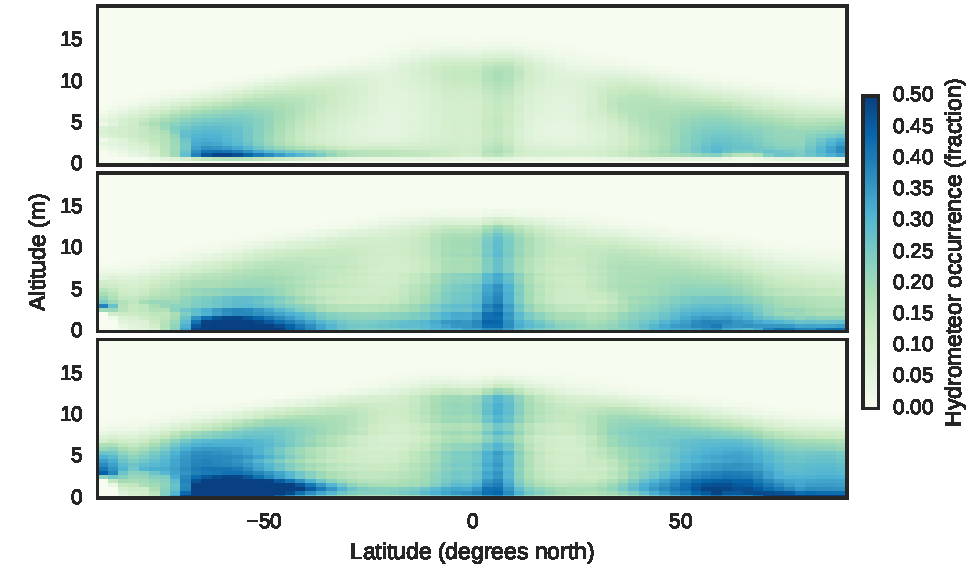
\includegraphics{graphics/cmip5_hfba.pdf}
\caption{\label{fig:cmip5_hfba}CloudSat hydrometeor occurrence
fraction.}\label{fig:cmip5ux5fhfba}
\end{figure}

\begin{figure}[htbp]
\centering
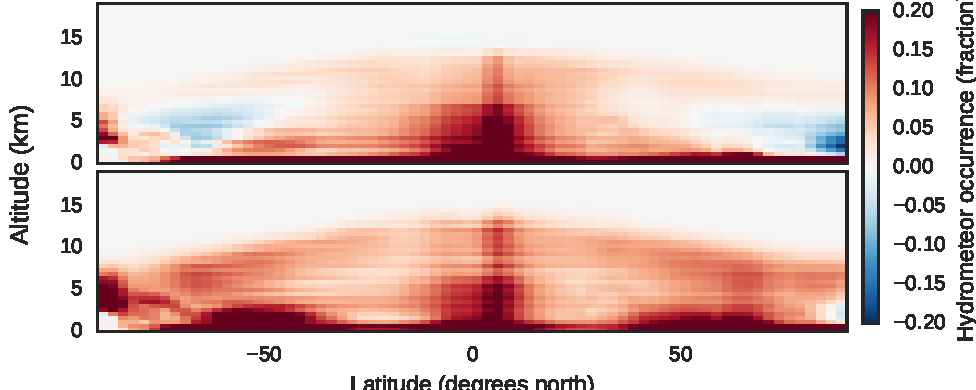
\includegraphics{graphics/cmip5_hfba_diff.pdf}
\caption{\label{fig:cmip5_hfba_diffs}CloudSat hydrometeor occurrence
fraction differences.}\label{fig:cmip5ux5fhfbaux5fdiffs}
\end{figure}

\begin{figure}[htbp]
\centering
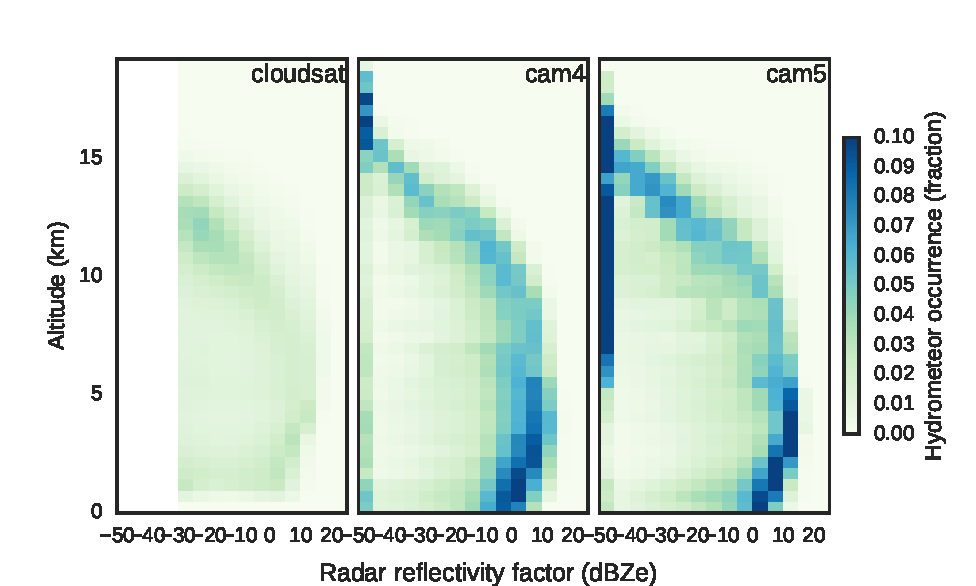
\includegraphics{graphics/cmip5_cfadDbze94_NHTropics.pdf}
\caption{\label{fig:cmip5_cfads}CloudSat
cfads.}\label{fig:cmip5ux5fcfads}
\end{figure}

\begin{figure}[htbp]
\centering
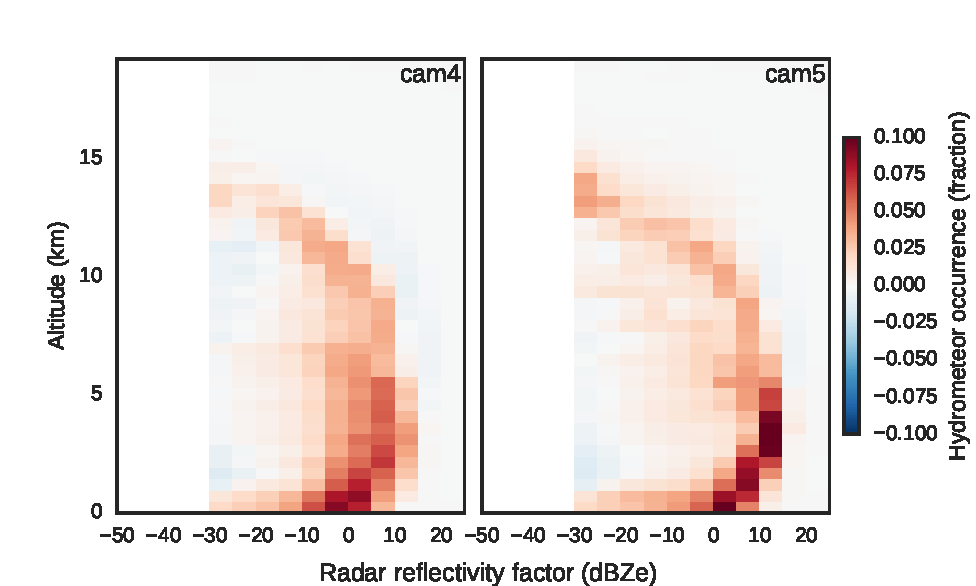
\includegraphics{graphics/cmip5_cfadDbze94_NHTropics_diff.pdf}
\caption{\label{fig:cmip5_cfads_diffs}CloudSat cfad differences relative
to CloudSat.}\label{fig:cmip5ux5fcfadsux5fdiffs}
\end{figure}

While the goal of the simulator framework is to remove uncertainties in
comparisons between models and observations by accounting for features
of the satellite retrievals, it is clear from the results presented here
that not all such uncertainties are removed with this framework, and
additional carefull interpretation of results is necessary.

Further points to make:

\begin{itemize}
\tightlist
\item
  Errors are on diagnostic side of model code, so errors do not
  necessarily represent errors in model parameterizations alone. Thus,
  care must be taken in interpreting these differences.
\item
  Errors are expected to arise due to using homogeneous cloud
  condensate, so models that do \emph{not} show these errors may have
  compensating errors, or erroneously tuned these errors out.
\item
  Errors in cloud area that arise due to using homogeneous cloud
  condensate are consistent with errors in cloud radiative effects; this
  demonstrates the far-reaching importance of properly treating
  unresolved cloud properties in models. It is not just a diagnostic
  problem, but permeates other areas of the model as well (radiative
  transfer in this case) that can feed back on the model simulation
  itself.
\item
  Cloud area is probably not a robust metric for model performance, due
  to the ambiguity in diagnosing this quantity from models and retrieve
  a similar quantity from satellites
\end{itemize}

TODO: discuss the path forward. Statistical cloud schemes? Better cloud
metrics for models?
